%%% První kapitola

\chapter{Definice a vlastnosti Jonesova polynomu}

Vhodné věci tučně, Zmínit původní definici?, Nekonzistentní používání V(t), V? Dvojtečky po platí

Původní definice Jonesova polynomu vycházela z operátorových algeber. A že tady to je na lincích.
\section{Základní pojmy}

Při definování Jonesova polynomu je důležité rozlišovat mezi linkem a jeho diagramem. Link je vnoření ... Diagram je vhodné rovinné nakreslení nějaké linkové projekce, v němž je rozlišeno, jestli křížení vedou zvrchu nebo zespodu. Každý link má nekonečně mnoho diagramů.

V diagramu orientovaného linku rozlišujeme křížení s kladnou a zápornou orientací, viz obrázek.

\begin{figure}[h]  
\centering 
\begin{subfigure}[t]{0.4\linewidth}\centering
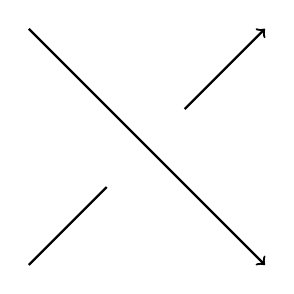
\begin{tikzpicture}[scale=3] 
\draw [thick] (0,0) -- (0.33,0.33);
\draw [thick,->] (0.66,0.66)-- (1,1);
\draw [thick,->] (0,1)  -- (1,0);
\end{tikzpicture} 
\caption{Kladná orientace} \label{fig:M1}  
\end{subfigure}
\begin{subfigure}[t]{0.4\linewidth}\centering
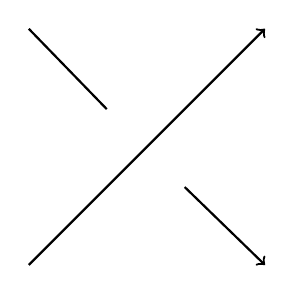
\begin{tikzpicture}[scale=3]
\draw [thick,->] (0,0) -- (1,1);
\draw [thick] (0,1) -- (0.33, 0.66);
\draw [thick,->] (0.66, 0.33) -- (1,0);
\end{tikzpicture}  
\caption{Záporná orientace} \label{fig:M2}  
\end{subfigure}
\caption{Orientace křížení}
\end{figure}  

Pro popis polynomů na uzlech a lincích se často používají tzv. skein (česky přadenové) vztahy.
Skein vztahy určují, jaká je spojitost mezi polynomy tří linků $L_+$, $ L_-$ a $L_0$, jejichž diagramy jsou identické až na oblast jednoho křížení. V linku $L_+$ má toto křížení kladnou orientaci, v $L_-$ zápornou a v $L_0$ je křížení rozpojené, viz obrázek.

\section{Definice}

\begin{definice}\label{def01:1}
Jonesův polynom orientovaného linku $L$ je Laurentův polynom v proměnné $\sqrt t$ (tj. polynom v $Z[\sqrt t, \sqrt{t^{-1}}]$), značený $V_L(t)$ , který
\begin{enumerate}[i.]
\item
je linkový invariant,
\item 
  je normalizovaný, tedy polynom  $V_\circlearrowleft$ triviálního uzlu má hodnotu $1,$
\item  
splňuje skein vztah 
$$ \frac{1}{t} V_{L_+} - t V_{L_-} = (\sqrt{t}  - \frac{1}{\sqrt{t}}) V_{L_0}.$$
\end{enumerate}
\end{definice}

\begin{lemma}
Buď $L$ link, který se skládá z $k$ neprotínajících se orientovaných triviálních uzlů. Pak $V_L(t) = (- \sqrt{t} -\frac{1}{\sqrt{t}} )^{k-1}	$.
\end{lemma}
\begin{dukaz}
Libovolně orientované triviální linky jsou ekvivalentní, stačí tedy vztah dokázat na diagramu zobrazujícím $k$ souhlasně orientovaných disjunktních kružnic.\\
Pro $k = 2$ je $L_0 = $, $L_- = $ a $L_+ = $. Diagramy $L_+$ a $L_-$ zobrazují triviální uzly, takže $V_{L_+} = V_{L_-} = 1$. Použitím skein vztahu získáme $V_ L = V_{L_0} = - \sqrt{t} -\frac{1}{\sqrt{t}} 	$. \\
Pro $k > 2$ jsou $L_-$ a $L_+ $ diagramy linků s $k-1$ kružnicemi, ze skein vztahu dostaneme $V_ L = V_{L_0} = (- \sqrt{t} -\frac{1}{\sqrt{t}} )^{k-1}$.
\end{dukaz}  
\begin{pozn}
Z každého diagramu uzlu lze změnou několika křížení vedených zvrchu na křížení vedených zespodu získat diagram triviálního uzlu. Z každého diagramu linku tedy můžeme změnou křížení získat diagram sjednocení triviálních uzlů, jejichž Jonesův polynom je podle předchozího lemmatu známý. Jonesův polynom každého linku lze tedy pomocí skein vztahu rekurzivně spočítat z jeho libovolného diagramu. Definice je tím pádem korektní.
\end{pozn}

Definice Jonesova polynomu pomocí skein vztahů není vhodná pro algoritmický výpočet, neboť rozpoznat, jestli diagram odpovídá triviálnímu uzlu, je složitý problém. K výpočtu použijeme ekvivalentní definici založenou na použití tzv. závorkového polynomu.

\section{Závorkový polynom}
Závorkový polynom (taktéž Kauffmanova závorka, angl. bracket polynomial) je definován pouze pro diagramy neorientovaných linků (tedy nikoli pro samotné linky). 

\begin{definice}\label{def01:2}
Závorkový polynom neorientovaného diagramu $D$, značený $\langle D \rangle$, je Laurentův polynom v proměnné $A$ definovaný třemi odvozovacími pravidly:
\begin{enumerate}[i.]
\item
$ \langle \bigcirc  \rangle = 1$, kde $\bigcirc$ značí diagram s jednou komponentou bez křížení
\item
$ \langle$ 

\begin{tikzpicture}[scale=0.4]
\draw (0,0) -- (1,1);
\draw (0,1) -- (0.33, 0.66);
\draw (0.66, 0.33) -- (1,0);
\end{tikzpicture}   
$\rangle = A  \langle $
%vert
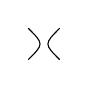
\begin{tikzpicture} [scale=0.4]
\draw (0,0) .. controls (1/2,1/2)  .. (0,1);
\draw (1,0) .. controls (1/2,1/2)  .. (1,1);
\end{tikzpicture}
$ \rangle + A^{-1}  \langle $
%hor 

\begin{tikzpicture} [scale=0.4]
\draw (0,0) .. controls (1/2,1/2)  .. (1,0);
\draw (0,1) .. controls (1/2,1/2)  .. (1,1);
\end{tikzpicture}
$\rangle $, kde $krizeni$ značí diagram obsahující křížení; $vert$ je diagram, který je shodný až na dané křížení, které je zde vertikální rozpojeno; a $hor$ je diagram, v němž je křížení rozpojeno horizontálně.
\item
$ \langle D \cup \bigcirc \rangle = (-A^2 - A^{-2}) \langle D \rangle$, kde $D \cup \bigcirc $ značí sjednocení diagramu $D$ a diagramu s jednou komponentou bez křížení.
\end{enumerate}


\end{definice}

\begin{dusl}
$ \langle $ 

\begin{tikzpicture}[scale=0.4]
\draw (0,0) -- (0.33,0.33);
\draw  (0.66,0.66)-- (1,1);
\draw (0,1)  -- (1,0);
\end{tikzpicture} 
$ \rangle = A  \langle $
%hor 

\begin{tikzpicture} [scale=0.4]
\draw (0,0) .. controls (1/2,1/2)  .. (1,0);
\draw (0,1) .. controls (1/2,1/2)  .. (1,1);
\end{tikzpicture}
$ \rangle + A^{-1}  \langle $
%vert
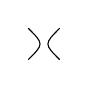
\begin{tikzpicture} [scale=0.4]
\draw (0,0) .. controls (1/2,1/2)  .. (0,1);
\draw (1,0) .. controls (1/2,1/2)  .. (1,1);
\end{tikzpicture}
$ \rangle $
\end{dusl}





\begin{lemma}  
Pro závorkové polynomy linků, jejichž diagramy obsahují smyčku, platí
\begin{enumerate}[i.]
\item
$ \langle $
%smycka 
\begin{tikzpicture}[baseline =\dimexpr-\fontdimen22\textfont2, scale = 0.25]
\begin{knot}[
consider self intersections=true,
clip width = 4,
end tolerance=1pt,
] 
\strand (0,-1) .. controls (3,3) and (3,-3) ..  (0,1);
\end{knot}
\end{tikzpicture}
$\rangle = -A^{-3} \langle $
%odsmycka
\begin{tikzpicture}[baseline =\dimexpr-\fontdimen22\textfont2,scale = 0.25]
\draw (0,1) .. controls (2.5,0) ..  (0,-1);
\end{tikzpicture}
$  \rangle$ 

\item
$ \langle $
\begin{tikzpicture}[baseline =\dimexpr-\fontdimen22\textfont2,scale = 0.25]
\begin{knot}[
consider self intersections=true,
clip width = 4,
end tolerance=1pt,
] 
\strand (0,1) .. controls (3,-3) and (3,3) ..  (0,-1);
\end{knot}
\end{tikzpicture}
$  \rangle = -A^{3} \langle $
%odsmycka
\begin{tikzpicture}[baseline =\dimexpr-\fontdimen22\textfont2,scale = 0.25]
\draw (0,1) .. controls (2.5,0) ..  (0,-1);
\end{tikzpicture}
$ \rangle$
\end{enumerate}
\end{lemma}

\begin{dukaz}
\begin{enumerate}[i.]
\item
$ \langle $
%smycka 
\begin{tikzpicture}[baseline =\dimexpr-\fontdimen22\textfont2, scale = 0.25]
\begin{knot}[
consider self intersections=true,
clip width = 4,
end tolerance=1pt,
] 
\strand (0,-1) .. controls (3,3) and (3,-3) ..  (0,1);
\end{knot}
\end{tikzpicture}
$\rangle =  A \langle $
%odsmycka
\begin{tikzpicture}[baseline =\dimexpr-\fontdimen22\textfont2,scale = 0.25]
\draw (0,1) .. controls (2.5,0) ..  (0,-1);
\end{tikzpicture}
$ \bigcup \bigcirc \rangle + A^{-1} \langle$  
%odsmycka
\begin{tikzpicture}[baseline =\dimexpr-\fontdimen22\textfont2,scale = 0.25]
\draw (0,1) .. controls (2.5,0) ..  (0,-1);
\end{tikzpicture}
$\rangle  = A (-A^2 - A^{-2})  \langle$  
%odsmycka
\begin{tikzpicture}[baseline =\dimexpr-\fontdimen22\textfont2,scale = 0.25]
\draw (0,1) .. controls (2.5,0) ..  (0,-1);
\end{tikzpicture}
$\rangle+ A^{-1}  \langle$  
%odsmycka
\begin{tikzpicture}[baseline =\dimexpr-\fontdimen22\textfont2,scale = 0.25]
\draw (0,1) .. controls (2.5,0) ..  (0,-1);
\end{tikzpicture}
$\rangle = -A^{-3} \langle $
%odsmycka
\begin{tikzpicture}[baseline =\dimexpr-\fontdimen22\textfont2,scale = 0.25]
\draw (0,1) .. controls (2.5,0) ..  (0,-1);
\end{tikzpicture}
$  \rangle$ 
\item
Analogicky.
\end{enumerate} 
$ $
\end{dukaz}

Dva diagramy znázorňují stejný link (jsou ekvivalentní), pokud mezi nimi existuje série Reidemeisterových pohybů (kde dokázané? + obrázek). Předchozí lemma říká, že závorkový polynom není invariantní vůči Reidemeisterovu pohybu typu I. Je ovšem invariantní Reidemeisterovým pohybům typu II a III.

\begin{tvrz}
Závorkový polynom je invariantní vůči Reidemeisterovým pohybům typu II a III.
\end{tvrz}
\begin{dukaz}
Par obrazku
Pak důsledek
\end{dukaz}

Aby byl závorkový polynom invariantní i vůči Reidemeisterovu pohybu typu I, je nutné vynásobit ho výrazem, který vyjadřuje míru zakroucení.

\begin{definice}
Zakroucení (writhe) orientovaného diagramu $D$ je součet znamení všech křížení v $D$. Zakroucení značíme $w(D)$.
\end{definice}

\begin{lemma}
Zakroucení je invariantní vůči Reidemeisterovým pohybům typu II a III.
\end{lemma}
\begin{dukaz}
Důkaz se provede rozborem případů.
\end{dukaz}

\begin{definice}
Normalizovaný závorkový polynom $X_L(A)$ orientovaného linku $L$ definijeme $X_L(A) = (-A^3)^{-w(D)}\langle D \rangle$, kde $D$ je libovolný diagram linku $L$.
\end{definice}

Definice je korektní, neboť následující tvrzení ukazuje, že nezáleží na volbě diagramu.

\begin{tvrz}
Normalizovaný závorkový polynom je linkový invariant.
\end{tvrz}
\begin{dukaz}
Závorkový polynom i zakroucení jsou invariantní vůči Reidemeisterovým pohybům typu II a III, invarientní je tedy i jejich součin.

Invariance vůči typu I plyne z Lemmatu 2 a faktu, že křížení v  
\begin{tikzpicture}[baseline =\dimexpr-\fontdimen22\textfont2, scale = 0.25]
\begin{knot}[
consider self intersections=true,
clip width = 4,
end tolerance=1pt,
] 
\strand (0,-1) .. controls (3,3) and (3,-3) ..  (0,1);
\end{knot}
\end{tikzpicture}
je vždy kladné a křížení v 
\begin{tikzpicture}[baseline =\dimexpr-\fontdimen22\textfont2,scale = 0.25]
\begin{knot}[
consider self intersections=true,
clip width = 4,
end tolerance=1pt,
] 
\strand (0,1) .. controls (3,-3) and (3,3) ..  (0,-1);
\end{knot}
\end{tikzpicture} záporné.
\end{dukaz}

\begin{veta}
Při substituce proměnné $A = t^{1/4}$ je normalizovaný závorkový polynom $X_L(A)$  roven Jonesovu polynomu $V_L(t)$.
\end{veta}
\begin{dukaz}
Ověříme, že $X_L(t^{1/4})$ splňuje podmínky v Definici 1.

\begin{enumerate}[i.]
\item
Podle předchozího tvrzení je linkový invariant.
\item
$X_\circlearrowleft = (-A^3)^0 \langle \bigcirc  \rangle = 1$ 
\item
fd
\end{enumerate}
$ $
\end{dukaz}



Vlastnosti:
uzly mají jen celočíselné, Amphichiral knots, 

Zminit, jake polynomy jsou zobecněním Jonesova?

Měla bych také říct, že je otevřená otázka, jestli má nějaký ne unknot polynom jedna.